\section{Shielding a \Libos{}}
\label{sec:sgx:shield}


\issuedone{1.1.d}{describe the security isolation story for SGX}
This section discusses how \graphenesgx{}
implements and shields the Linux ABI for applications in enclaves.

%\fixmedp{RC: Please print this in black and white, and make sure it looks
%  ok wihtout red/green on the figures.}

%the components of the \graphenesgx{} framework designed for isolating single-process applications in \sgx{} enclaves, and the design of the OS shielding layer against the untrusted hosts.


\subsection{Shielding dynamic loading}
\label{sec:sgx:shield-loading}


%\graphenesgx{} secures Linux COTS applications without any modification and recompilation.
To run unmodified Linux binaries,
\graphenesgx{} implements dynamic loading and run-time linking.
%, with the integrity protection of SGX.
In a major Linux distribution like Ubuntu, more than 99\% of binaries are dynamically linked~\cite{tsai16apistudy}.
%\fixmedp{Please check this}
Static linking is popular for SGX frameworks because it is simple and 
facilitates the use of hardware enclave measurements. %, and requires no extra shielding against malicious binaries. % by the hardware at start time.
%the hardware
%can measure the integrity of an enclave at start time.
%\fixmedp{Check my edit of the next sentence}
Dynamic linking requires rooting trust in a dynamic loader, which must then measure the libraries.
For Haven~\cite{baumann14haven}, the enclave measurement only verifies the integrity of Haven itself,
%and Haven loads the binaries from an encrypted archive.
and the same measurement
applies to any application running on the same Haven binary.
%executables and libraries that requires dynamic linking~
%The dynamic linking behavior of Linux applications allows sharing the libraries among the run-time executables,
%reducing the disk space for storing all binaries and the deployment cost for upgrading libraries.
%Moreover, a dynamically-linked library can be selectively loaded by an application, thus reducing the TCB when the application requires no functionality from the library.
%Due to the ubiquity of dynamically-linked binaries,
%\graphenesgx{} has to shield the dynamic linking behavior in order to support most of the Linux COTS applications.



%Because the majority of Linux executables dynamically link against shared libraries and plug-in modules,
%new challenges emerge in reproducing the code integrity and authentication properties of \sgx{} enclaves.
%Formerly, an enclave is expected to have a static code footprint
%so that the \intel{} CPU can generate a signed attestation for the authenticity of the execution.
%\sgx{} \libos{}es such as \haven{}
%securely loads application binaries after enclave creation
%because the initial enclave code, the shielding layer, is fully trusted by the clients.




\begin{comment}
When \graphenesgx{} isolates a Linux COTS application,
it allows remote entities to differentiate the execution from other applications, 
without relying the uniqueness of signing keys or software vendor IDs.
Instead, \graphenesgx{} creates enclaves using the cryptographic measurements (application signatures)
that are unique to the results of dynamic linking.
If any part of the linked executables and libraries become different,
the measurement will reflect the difference and it is computationally infeasible to brute-forcely find another dynamic linking result that leads to the same measurement.
\end{comment}




%If the initial code can securely load new code into the enclave
%if the initial code is trusted to verify and attest the newly loaded code throughout the lifetime of the enclave.
%For instance, \haven{} dynamically loads the \libos{} and application binaries
%but can still be trustworthy because \haven{} retrieves the binaries from an encrypted virtual disks. The chain of trust for applications secured by \haven{] }is built upon the same client signing both the \haven{} enclaves and the key-provisioning server.



%For each binary loaded by \graphenesgx{}, \graphenesgx{} bootstraps the enclave
%from an untrusted platform adaption layer (PAL) that defines
%a narrowed untrusted interface.
%To speed up initialization, the untrusted PAL starts the enclave
%with an statically linked library image ({\tt graphene.so}).
%The image includes
%\graphene{} host ABI,
%\libos{} ({\tt libLinux}, implementing Linux personality),
%and basic libraries of glibc
%({\tt libc}, {\tt libpthread} and {\tt ld}, the runtime loader).
%The \graphenesgx{} library image then loads the unmodified applications
%and libraries into the enclave.

\graphenesgx{} extends the Haven model to generate a unique signature for
any combination of executable and dynamically-linked libraries.
Figure~\ref{fig:sgx:arch} shows the architecture and the dynamic-loading process
of an enclave. % created by \graphenesgx{}.
\graphenesgx{} starts with an untrusted Platform Adaption Layer ({\tt pal-sgx}), which calls the SGX drivers to initialize the enclave.
%interacts with the \graphenesgx{} driver and the \intel{} \sgx{} driver to
%initiate the enclave.
%Each enclave created by \graphenesgx{} is equivalent to a process of an application.
The initial state of an enclave, which determines the measurement then 
attested by the CPU, includes a shielding library ({\tt libshield.so}),
the executable to run,
and a manifest file that specifies the attributes and loadable binaries in this enclave.
The shielding library then loads a Linux library OS ({\tt libLinux.so}) and the standard C libraries ({\tt ld-linux-x86-64.so} and {\tt libc.so}).
After enclave initialization, the loader continues loading
additional libraries, which are checked by the shielding libraries.
If the SHA-256 hash does not match the manifest, the shield will refuse
to open the libraries.

%Each library loaded after enclave initialization, the files are checked by the shielding library against the SHA-256 hashes stored and signed in the manifest.
%The shield will refuse to load  libraries that do not have a matching hash in the manifest.


\begin{figure}[t!]
\centering
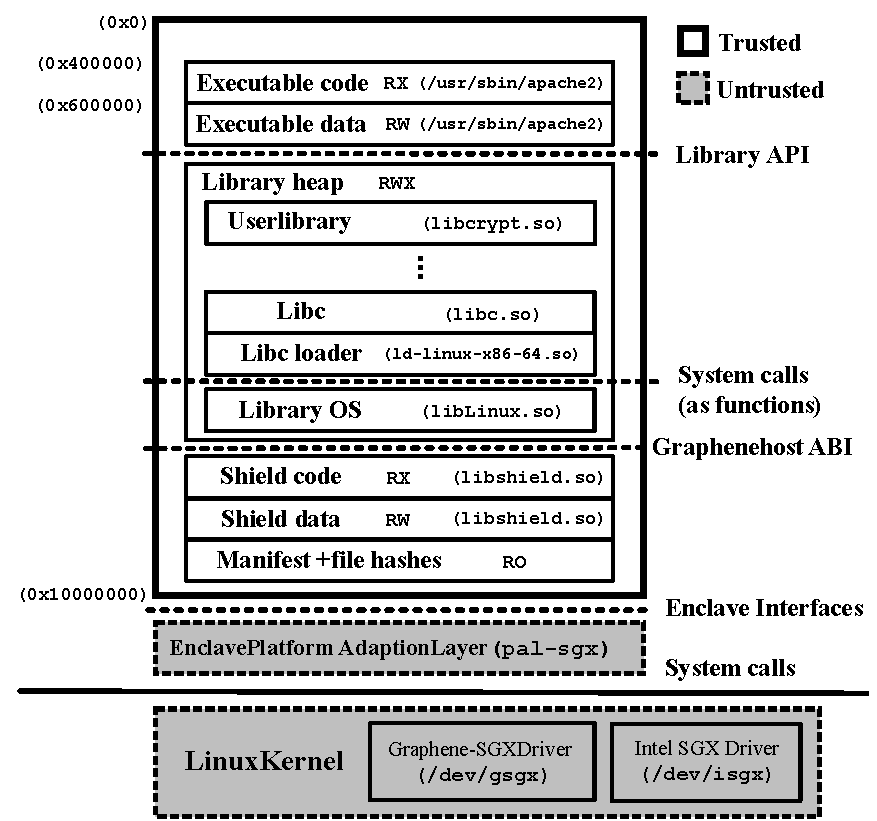
\includegraphics[width=.75\linewidth]{architecture.pdf}
\caption{The \graphenesgx{} architecture. The executable is position-dependent.
%The enclave size is 16MB. % (highest at 0x10000000).
The enclave includes an OS shield, a library OS, libc, and other user binaries.
%libc and other shared libraries, and the executable, all of which are secured with binary integrity.
%% dp: meh
%The integrity of these binaries is validated by either the CPU or the shield.
%\graphenesgx{} also uses kernel drivers, but does not trust them.
}
%\graphenesgx{} is statically linked with {\tt libLinux},
%the \libos{} binary, and basic libraries of GNU library C.
%To build up the trust, the \graphenesgx{} image along with
%a manifest and application measurements
%are verified by \sgx{} during bootstrap. Applications and other libraries
%are verified by \graphenesgx{}. The enclave interacts with the host kernel,
%through untrusted PAL, on a narrowed untrusted interfaces with xx functions.}
\label{fig:sgx:arch}
\end{figure}


To reiterate, a manifest includes integrity measurements of all components and is signed; this manifest is unique for each application and is measured as
part of enclave initialization. %, generating a unique measurement for each application.
This strategy does require
trust in the Graphene (in-enclave) bootloader and shielding module to correctly load binaries
according to the manifest and reject any errant binaries offered by the OS.  This is no worse than the level trust
placed in Haven's dynamic loader, but differentiates applications or even instances of the same application with different libraries.


%enforces a {\em white-list} policy for dynamic loading---only libraries that have a matching checksum in the manifest can be loaded into the enclave.



%%The structure of an enclave created by \graphenesgx{} contains
%%the native application executables and libraries, the upstream \graphene{} \libos{} (libLinux.so) and an OS shield for validating input resources to the enclave interface (as figure~\ref{fig:arch}).
%%A building block of the \graphenesgx{} run-time framework is structured as  figure~\ref{fig:arch} reveals.
%Each enclave of \graphenesgx{} equals to a process of regular execution,
%but with the end-to-end isolation of an \sgx{} enclave.
%The whole virtual memory address space of the application process
%and most of the \graphenesgx{} runtime reside inside the range of enclave memory,
%thus being completely isolated from external access.
%Only a thin translation layer executes outside the enclave in the user-space,
%and its purpose is to translate the enclave interface to host system APIs.
%For clarification, we will refer to the enclave which mimics a process of the isolated application as an {\bf enclave process},
%in the contrary with a {\bf host process}---which the untrusted host OS creates and sees.



\begin{comment}
To summarize,
\graphenesgx{} enforces the integrity of an application loaded into an enclave based on two strategies:
First, the shielding library and the executable to run are verified as part of the cryptographically-measured memory. 
Second, the Linux library OS, the standard C libraries,
and other user libraries are verified against the checksums stored in a manifest,
which is also part of the measured memory.
The measurement is essentially a message authentication code (MAC) of the isolated application,
and a MAC that authenticates checksums generated by a secure hashing algorithm like SHA-256 is equally indistinguishable as a MAC that directly authenticates the checksum'ed binaries.
\end{comment}





%Each enclave launched in \sgx{} requires a signature, signed by developers.
%The signature structure ({\tt SIGSTRUCT}) contains
%enclave attributes, product ID, a public key, enclave measurement
%and RSA-based signature of the structure.
%\graphenesgx{} maintains enclave signatures on a per-binary basis.
%Unlike \haven{}, we extend the enclave's measurement to
%cover all binaries loaded in the enclave, not just the \libos{} itself.
%To keep the application binaries being dynamically loaded,
%the measurement of these binary files are stored as
%{\bf application checksums}, verified by \graphenesgx{} at loading.
%With the application checksums being measured in enclaves,
%different binaries loaded with different library dependencies
%will naturally yield different measurements,
%easily differentiating the attestations generated by processors.

%\paragraph{Relocation and resolution.}
%Dynamic linking is not a completely deterministic process;
%ASLR (address space layout randomization) in the library OS
% and run-time linking functions (e.g., {\tt IFUNC} symbols)
%can lead to variations in the address space composition.
%\graphenesgx{} generates a summary of the linking results,
%%extends the remote attestation report generated by hardware with a
%%summary of the linking results, 
%including the Global Offset Tables (GOTs) of the loaded binaries,
%which can be attached in remote attestation reports.
%%This summary is digitally signed by \graphenesgx{} to further attest that a sensible in-memory binary
%%was linked at runtime.

%% Note that the loaded binaries are not the only factors that determine the run-time executables.
%% Even if the loaded binaries are exactly the same,
%% the process of dynamic linking may result in different linking results,
%% due to ASLR (address space layout randomization) in library OS or run-time linking functions ({\tt IFUNC} symbols).
%% To include these information in the attestation,
%% \graphenesgx{} generates a summary of the
%% linking results, including the copies of Global Offset Tables (GOTs) of the loaded binaries.
%% The summary is digitally signed and attached with the CPU-generated attestation reports.



\paragraph{Memory permissions.} %\fixmedp{please check}
By default, the Linux linker format (ELF) often places
code and linking data (e.g., jump targets) in the same page.
It is common for a library to temporarily mark an executable pages as writable
during linking, and then protect the page to be execute-only.
This behavior is ubiquitous in current Linux shared libraries, but could be changed at compile time to pad
writable sections onto separate pages.

The challenge on version 1 of SGX is that an application cannot revoke page
permissions after the enclave starts.
In order to support this ELF behavior, we currently map all enclave pages
as readable, writable, and executable.
This can lead to some security risks, such as code injection attacks in the enclave.
In a few cases, this can also harm functionality; for instance, some Java VM implementations
use page faults to synchronize threads.
Version 2 of SGX~\cite{sgx2} will support changing page protections,
which \graphenesgx{} will adopt in the future. % versions of \graphenesgx{}.


\begin{comment}
The current version of SGX hardware requires the maximum enclave size to be specified at initialization time.
Thus, \graphenesgx{} also allows the user to specify a reserved heap size,


has to reserve a heap space in each enclave, in order to load application binaries
or to create anonymous mappings.
The in-enclave heap needs to have full access permissions, as readable, writable, and executable,
to be dynamically allocated as user memory mappings.
On current x86/64 architecture, memory permissions cannot be revoked after enclave creation.
Retaining full access permissions on the whole in-enclave heap can cause security issues, such as code injection or reusing data sections as {\em gadgets}.
We expect this vulnerability will be fixed on \sgx{}2~\cite{sgx2}, the next-generation \sgx{} hardware, which provides new instructions to support dynamic memory protection.
In general, making the heap readable, writable, and executable does not hurt compatibility, besides some applications like JVM runtimes that rely on protecting memory to synchronize.
\end{comment}



%Although \haven{} only includes the shielding module
%in the enclave measurements,
%it can still differentiate applications by forcing different digests
%on the same shielding module.
%The trick is to inject an unique ID for each application,
%into the module binary.
%We argue that \graphenesgx{} uses a more straightforward model, with no need to
%maintain the uniqueness of any IDs.

\paragraph{Position-dependent executables.}
SGX requires that all enclave sizes be a power-of-two,
and that the enclave starts at a virtual address aligned to the enclave size.
Most Ubuntu Linux executables are compiled to be position-dependent, and typically 
start at address 
{\tt 0x400000}.  The challenge is that, to create an enclave  that includes this address and is larger than 4MB, the enclave
will necessarily need to include address zero.
% \fixmedp{I thought the offending address was 64K.., not {\tt 0x400000}}.

%As part of the Linux convention, most executables are compiled as position-dependent, starting at address {\tt 0x400000} by default.
%To support these executable, \graphenesgx{} must create enclaves with the base address {\tt 0x0}.
%The existence of position-dependent executables forces \graphenesgx{} to create enclaves that include specific addresses.
%To support these executable, \graphenesgx{} creates enclaves that explicitly starts at address {\tt 0x0}.
%This restriction is due to
%One reason for starting the enclaves at {\tt 0x0} is due to 
%the hardware prerequisite to align enclave base address to enclave sizes.

We see including address zero in the enclave as a net positive, but not strictly necessary, as we are reluctant to make strong claims 
in the presence of code that follows null pointers.
\graphenesgx{} can still mark this address as unmapped in an enclave.
% ensure that this address remains unmapped inside the enclave by memory protection of \sgx{}.
Thus, a null pointer will still result in a page fault.
On the other hand, if address zero were outside of the enclave,
there is a risk that the untrusted OS could map this address to dangerous data~\cite{cve-2009-2692},
undermining the integrity of the enclave.
% \fixmedp{Can you actually execute non-enclave code without an ocall?  I assume not...}
 
 
% Basing the enclave at {\tt 0x0} also prevent an attack
%exploiting application vulnerabilities that reference {\tt NULL} pointers~\cite{cve-2009-2692}.
%\graphenesgx{} preserves the first pages of each enclave as inaccessible to prevent this attack.

 





\subsection{Shielding \thehostabi{}}
\label{sec:sgx:shield-abi}


%\begin{figure*}
%\footnotesize
\centering
\bgroup
\def\arraystretch{1.1}
%\setlength{\tabcolsep}{0.5em}
\begin{tabular}{|>{\raggedright\arraybackslash}p{12em}|>{\centering\arraybackslash\bf}p{4em}|>{\centering\arraybackslash}p{4em}|>{\centering\arraybackslash}p{4em}|>{\centering\arraybackslash}p{4em}|}
\hline
Classes                         & Safe & Benign & DoS & Unsafe \\
\hline
\hline
Enter enclaves \& threads       & 2    & 0      & 0   & 0     \\
% start_enclave     (safe)
% start_thread      (safe)
\hline
Clone enclaves \& threads       & 2    & 0      & 0   & 0     \\
% create_process    (safe)
% create_thread     (safe)
\hline
File \& directory access        & 3    & 0      & 0   & 2     \\
% file_open         (safe)
% file_truncate     (safe)
% file_stat         (unsafe)
% dir_read          (unsafe)
\hline
Exit enclave                    & 1    & 0      & 0   & 0     \\
% thread_exit       (safe)
\hline
Network \& RPC streams          & 5    & 2      & 0   & 0     \\
% sock_listen       (safe)
% sock_accept       (safe)
% sock_connect      (safe)
% sock_send         (safe)
% sock_recv         (safe)
% sock_setopt       (benign)
% sock_shutdown     (benign)
\hline
Scheduling                      & 0    & 1      & 1   & 0     \\
% yield             (benign)
% futex             (blockable)
\hline
Stream handles                  & 2    & 2      & 1   & 0     \\
% handle_close      (benign)
% handles_poll      (blockable)  
% handle_send       (safe)
% handle_recv       (safe)
% handle_flush      (begign)
\hline
Map untrusted memory            & 2    & 0      & 0   & 0     \\
% map_untrusted     (safe)
% unmap_untrusted   (safe)
\hline
Miscellaneous                   & 1    & 1      & 0   & 0     \\
% get_time          (safe)
% sleep             (benign)
\hline
\hline
{\bf Total}                     & 18   & 6      & 2   & 2     \\ 
\hline
\end{tabular}
\egroup

%\caption{The enclave interface of \graphenesgx{}.}
%%consisting of 17 functions to access host OS features when the \libos{} is insufficient to handle internally.
%%\graphenesgx{} shields its enclave interface from the untrusted host OS, assuming each input value of the interface to be potentially malicious.
%%Most of the enclave interface is inherited from the \graphene{} host ABI.}
%\label{tab:interface}
%\end{figure*}



%\graphenesgx{} is derived from \graphene{} \libos{}, which runs unmodified
%Linux applications ranged from Apache web servers to shell scripts.
%\graphene{} \libos{} originally runs on Linux hosts, but with the platform
%adaption layer (PAL) ported to other platform,
%\graphene{} can run Linux applications on other hosts such as
%Windows, BSD or OSX.
%\graphene{} supports up to 139 most commonly used Linux system calls
%(300 in total),
%providing reasonable Linux platform compliance.



For a single-process application running on \graphenesgx{},
most Linux system calls are serviced inside the enclave by the library OS.
A \graphenesgx{} enclave includes both the same library OS 
in ``classic'' Graphene, that would also run on a Linux or FreeBSD picoprocess,
% (which runs natively in a Linux or FreeBSD process) in the enclave,
as well as an SGX-specific platform adaptation layer (PAL), 
which implements \palcallnum{} functions of the host ABI that the library OS is programmed against.
This PAL funnels to a slightly smaller set of
%Between the enclave and untrusted code is a even simpler interface, that contains 
\enclavecallnum{} interfaces which the enclave calls out to the untrusted OS (Table~\ref{tab:sgx:enclave-abi}).
%, summarized in Table~\ref{tab:interface}.
%Table~\ref{tab:interface} lists the \enclavecallnum{} entries of the enclave interface defined in \graphenesgx{}.

%% \graphenesgx{} can isolate the Linux system calls used by the application, encapsulated by the \libos{} accompaning the application in the enclave.
%% Using a \libos{} retains most of the OS states and activities inside the enclaves, keeping the interaction with the untrusted host OSes to the minimum---only when requesting an abstraction managed by the host OSes or sharable among applications. When interacting with the host OSes, \graphenesgx{} uses an enclave interface derived from the narrowed host ABI inherited from the \graphene{} \libos{}~\cite{tsai14graphene}, which contains \palcallnum{} host functions.
%% \graphenesgx{} does not directly export the \graphene{} host ABI; instead, it defines an even narrower and simpler enclave interface below the host ABI, to ensure that the whole enclave interface can be properly shielded.





%Due to the limitation of \sgx{},
%the starting address and the size of an enclave process are static since the enclave creation.
%The pre-defined enclave range written in the manifest is immutable after being signed by trusted entities.
%The range must be large enough to cover the mapping regions of position-dependent binaries. As a convention followed by most Linux applications, the majority of executable binaries are compiled with fixed mapping addresses, commonly at {\tt 0x400000} (the code segment) and {\tt 0x600000} (the data segment).


%To support position-dependent executables, \graphenesgx{} initiates all enclaves to start at the address {\tt 0x0}.
%This setup is due to the limitation that \sgx{} requires each enclave to start at an address to be power of two, and the enclave size to be a factor of its start address.
%According to this limitation, unless the memory size needed by an executable located at {\tt 0x400000} is less than 4MiB, the enclave must start at {\tt 0x0} instead of {\tt 0x400000}.



%Table~\ref{tab:interface} lists the \enclavecallnum{} entries of the enclave interface defined in \graphenesgx{}.
%We show that the enclave interface is sufficient to implement most of the \palcallnum{} functions
%in the \graphene{} host ABI (except 5 optional PAL ABIs for optimization and sandboxing only).
%These enclave calls are sufficient to run the \libos{} ({\tt libLinux.so}) to implement the Linux personality.
%The sufficiency of the enclave interface is essential to reusing the development effort of the \graphene{} \libos{}.



%As part of each enclave process, 
%the \graphenesgx{} run-time framework consists of an OS shield ({\tt libshield-sgx.so}), a \graphene{} \libos{} ({\tt libLinux.so}),
%an intercepted version of GNU library C ({\tt libc} and {\tt ld.so})---all to support and secure the execution of an unmodified Linux application.
%The interfaces to these components are marked in Figure~\ref{fig:arch}.
%The intercepted {\tt libc} and {\tt ld.so} provides the standard C library functions for the application and its supporting libraries.
%The \graphene{} \libos{} supports the native Linux system calls for {\tt libc} and {\tt ld.so}.
%The OS Shield supports the host ABI functions used in the \libos{} implementation, and exports the shielded enclave interface to the untrusted host.
%In this design, the OS Shield is only part of the enclave whose implementation is unique to \sgx{}, the rest of the enclave is directly inherited from a regular \graphene{} picoprocess, so it can receive any upstream fixes on the \libos{} ({\tt LibLinux.so}) from the \graphene{} project.


%\fixmedp{my attempt to crispen this point; CC: see what you think.  The read
%example isn't sending me}
The evolution of the POSIX API and Linux system call table
were not driven by a model of mutual distrust, and retrofitting
protection onto this interface is challenging.
Checkoway and Shachman~\cite{checkoway13iago} demonstrate 
the subtlety of detecting semantic attacks via the POSIX interface.
%called Iago attacks.
Projects such as Sego~\cite{kwon2016sego} go to significant lengths, including
modifying the untrusted OS, to validate OS behavior on subtle and idiosyncratic
system calls, such as \syscall{mmap} or \syscall{getpid}.
% semantics attacks, from an untrusted OS, on the POSIX or Linux system call table as is (i.e., Iago attacks).
%Both SCONE~\cite{osdi16scone} and Panoply~\cite{shinde17panoply} defends applications from memory-based Iago attacks, by checking pointers returned by a Linux system call or a POSIX function to be outside the enclave.
%However, to defend more subtle semantics, such as the stateful {\tt read()}, both shim layers have to pull more state into the enclave and simulate the behaviors of a trusted OS. To check {\tt read()}, one has to maintain a pointer to the current offset of the file descriptor, which has to be incremented at every {\tt read()} and its variants (e.g., {\tt readv()}), and affected by the arbitrary-length data that an OS can lawfully return.

%{\bf What is an enclave interface amenable for shielding applications?}
%\graphenesgx{} shields each of these 28 interfaces at the enclave boundary
%to detect malicious inputs from the host OS, i.e., Iago attacks~\cite{checkoway13iago}).
The challenge in shielding an enclave interface is carefully
defining the expected behavior of the untrusted system,
and either validating the responses, or reasoning that any response 
cannot harm the application.
By adding a layer of indirection under the library OS, we can define
an enclave ABI that has
%One advantage of using a library OS is that one can define an enclave ABI that has
more predictable semantics, which is, in turn, more easily checked at run-time.
%In general, it is difficult to completely defend against Iago attacks on the existing system APIs
%due to the complexity.
%However, with a \libos{} to translate the system APIs for applications, we can redefine the enclave interface to make the inputs much more predictable and thus easier to velidate.
For instance, to read a file, \graphenesgx{} requests that untrusted OS to map the file at an address outside the enclave, starting at an absolute offset in the file, with the exact size that the library OS needs for checking.
After copying chunks of the file into the enclave, but before use, the contents can be hashed and checked against the manifest.
%To prevent Iago attacks, \graphenesgx{} can predict the input returned by this specific request,
%which is a buffer outside the enclave storing part of the file.
%Since Iago attacks can happen randomly and are often unpredictable, \graphenesgx{} must assume all inputs to each entry to be potentially malicious, and only accept the inputs as predicted. when reading the file content at an absolute offset, it is easy to match the input with the checksums generated from chuncks %of the files.
%On the contrary, if the interface to shield is the Linux system call table or POSIX API, API variants like \funcname{read}, \funcname{readv}, and \funcname{aio\_read} will be more complex and unpredictable due to exporting OS states like file offsets to the untrusted OSes.
This enclave interface limits the possible return values to one predictable answer, and thus reduces the space that the OS can explore to find attack vectors to the enclave.
%\fixmedp{This example is ok, but a little weak; have one that is more prone to iago?}
Many system calls are partially (e.g., {\tt brk}) or wholly (e.g., \syscall{fcntl}), absorbed into the library OS, and do not need shielding from the untrusted OS.
%\fixmedp{getpid is also a little underwhelming, anything more sophisticated that is fully in the libos?}

%% dp: I think this is too down in the weeds, given our space constraints
\begin{comment}
\edit{To be clear, \graphenesgx{} can still have vulnerabilities in the shielding library if not implemented carefully. \fixme{Don, check this. Delete if you don't like it.} For instance, a vulnerability was discovered in a previous version of \graphenesgx{}, by Bulck, in the assembly code that checks and purges registers immediately after enclave entry~\cite{bulck-graphene} (the vulnerability is fixed later).
The principle of \graphenesgx{} on shielding applications is to preemptively check all inputs at the entrance,
so that the safety of our enclave interface does not have to rely on the correctness of the library OS.}
\end{comment}


\begin{table}
\footnotesize
\centering
\bgroup
\def\arraystretch{1.1}
\setlength{\tabcolsep}{0.5em}
\begin{tabular}{|>{\raggedright\arraybackslash}p{12em}|>{\centering\arraybackslash\bf}p{2.8em}|>{\centering\arraybackslash}p{2.8em}|>{\centering\arraybackslash}p{2.8em}|>{\centering\arraybackslash}p{2.8em}|}
\hline
Classes                         & Safe & Benign & DoS & Unsafe \\
\hline
\hline
Enter enclaves \& threads       & 2    & 0      & 0   & 0     \\
% start_enclave     (safe)
% start_thread      (safe)
\hline
Clone enclaves \& threads       & 2    & 0      & 0   & 0     \\
% create_process    (safe)
% create_thread     (safe)
\hline
File \& directory access        & 3    & 0      & 0   & 2     \\
% file_open         (safe)
% file_truncate     (safe)
% file_stat         (unsafe)
% dir_read          (unsafe)
\hline
Exit enclave                    & 1    & 0      & 0   & 0     \\
% thread_exit       (safe)
\hline
Network \& RPC streams          & 5    & 2      & 0   & 0     \\
% sock_listen       (safe)
% sock_accept       (safe)
% sock_connect      (safe)
% sock_send         (safe)
% sock_recv         (safe)
% sock_setopt       (benign)
% sock_shutdown     (benign)
\hline
Scheduling                      & 0    & 1      & 1   & 0     \\
% yield             (benign)
% futex             (DoS)
\hline
Stream handles                  & 2    & 2      & 1   & 0     \\
% handle_close      (benign)
% handles_poll      (DoS)  
% handle_send       (safe)
% handle_recv       (safe)
% handle_flush      (begign)
\hline
Map untrusted memory            & 2    & 0      & 0   & 0     \\
% map_untrusted     (safe)
% unmap_untrusted   (safe)
\hline
Miscellaneous                   & 1    & 1      & 0   & 0     \\
% get_time          (safe)
% sleep             (benign)
\hline
\hline
{\bf Total}                     & 18   & 6      & 2   & 2     \\ 
\hline
\end{tabular}
\egroup

\caption{\enclavecallnum{} enclave interfaces,
including {\em safe} (host behavior can be checked), {\em benign} (no harmful effects), {\em DoS} (may cause denial-of-service), and {\em unsafe} (potentially attacked by the host) interfaces.}
%\fixme{Not sure if we should list all enclave interface in detail.}}
%% dp: It would be nice to fully list, but I don't think we have space.
%consisting of 17 functions to access host OS features when the \libos{} is insufficient to handle internally.
%\graphenesgx{} shields its enclave interface from the untrusted host OS, assuming each input value of the interface to be potentially malicious.
%%Most of the enclave interface is inherited from the \graphene{} host ABI.}
\label{tab:sgx:enclave-abi}
\end{table}


Table~\ref{tab:sgx:enclave-abi} lists our \enclavecallnum{} enclave interfaces,
organized by risk.
%easily-checked semantics (safeith risk assessed by whether each of them has predictable semantic or robust defense strategy.}
%also assesses the risk of each enclave interface,
%based on how problematic a malicious input could be for the Library OS.
%We evaluate the security of the enclave interface in \graphenesgx{} based on the difficulty of verifying the inputs and the worst consequence of accepting malicious inputs, as shown in 
%More details of the security evaluation will be discussed in \S\ref{sec:eval:security}.
%The \enclavecallnum{} entries of the \graphenesgx{} enclave interface are categorized into four groups: There are
18 interfaces are {\em safe} because responses
from the OS are easily checked in the enclave.
An example of a safe interface is \funcname{FILE\_MAP},
which maps a file outside the enclave,
to copy it into the enclave for system calls like \funcname{mmap} or \funcname{read}, as discussed below.
%A pre-constructed secure hash can be mapped to the copied file to validate its integrity.
6 interfaces are {\em benign}, which means, if a host violates the specification,
the library OS can easily compensate or reject the response.
% will compensate appropriately or reject the outcomes.
An example of a benign interface is \funcname{STREAM\_FLUSH},
which requests that data be sent over a network or to disk;
cryptographic integrity checks on a file or network communication can 
detect
when this operation is ignored by untrusted software.
% cases where a 
%ignores requests to write data to disk or the network.
%trusting most host OSes to benignly serve the requests.
%However, if the host OSes maliciously reject serving these {\em benign} entries, no harm can be done, and \graphenesgx{} will discard any inputs from the host OSes.
%As an example of {\em benign} entries, \funcname{stream\_flush} requests the host OSes to flush the data written to a file or network connection, but does not rely on the host OSes to reliably serve the request, because there should be message authentication in place. Other two entries, \funcname{futex} and \funcname{stream\_poll} spefically, may be minimally corrupted by malicious inputs, but the worst consequences of the corruption is denial-of-the-service ({\em DoS}).


Like any SGX framework, \graphenesgx{} does not guarantee liveness of enclave code: the OS can refuse to schedule the enclave threads.
Two interfaces are susceptible to liveness issues (labeled {\em DoS}): \funcname{FUTEX\_WAIT} and \funcname{STREAM\_POLL}.
In the example of \funcname{FUTEX\_WAIT}, a blocking synchronization call may never return, violating liveness but not safety.
A malicious OS could cause a futex wait to return prematurely; thus, 
synchronization code in the PAL
must handle spurious wake-ups and either attempt to wait on the futex again, or spin in the enclave.
%{\em DoS} calls can be considered a subset of {\em benign}.
%Because the host OSes can anyway take away the CPU resource or block the network bandwidth to cause DoS attacks on enclaves, these two entries are not considered security threats to \graphenesgx{}. 

Finally, only two interfaces, namely \funcname{FILE\_STAT} and \funcname{DIR\_READ}, are {\em unsafe}, because we do not protect
integrity of file metadata.  We leave this issue
%protection of file system  metadata 
for future work, adopting one of several existing solutions~\cite{inktag}.
%~\fixmedp{cite: integrity protected FSes, and maybe Inktag iirc?}


%% dp: Meh
\begin{comment}
\begin{edits}
The justification of the safety of \graphenesgx{}'s enclave interface is as follows: 
(1) our enclave interface contains only \enclavecallnum{} functions, with only the simplest semantics and minimal corner cases, so is much easier to check than a significant portion of the Linux system call table or POSIX API. (2) for majority of these \enclavecallnum{} functions, the shielding library can either predict a single value that the OS is allowed to return, or completely dismiss any return values from the OS.
\end{edits}
\end{comment}
 
%Similar as \haven{} and \scone{}, 
%\graphenesgx{} secures the OS interaction of an application against known direct attacks from the untrusted host,
%by absorbing the OS components into the enclave and implementing upon a narrow enclave interface.
%The narrowness of the enclave interface facilitates the design of shielding strategies on the input resources of the enclave interface.
%The host abstractions exposed by the enclave interface is supposed to be a bare minimum, but sufficient to implement the Linux personality for the isolated applications.
%The enclave interface of \graphenesgx{} exports \enclavecallnum{} entry or exit functions, as listed in Figure~\ref{tab:interface},
%to be either shielded or untrusted by the enclave.
%More details of the shielding strategies for the internal system calls are discussed in \S\ref{sec:overview:shield}.


%The untrusted interface of \graphenesgx{} is defined as Table~\ref{tab:interface}.
%The Untrusted interface of an enclave is the API that communicates the enclave
%and the untrusted host, with both entries and exits of the enclave.
%Note that for hardware an enclave only has exactly one entry and exit,
%to which execution jumps
%using {\tt EENTER} and {\tt EEXIT} instructions.
%The untrusted interface is simply a callback table that redirects execution
%afterward (similar to system calls).







%\graphenesgx{} drops the enclave interface right above the translation layer
%to the host system APIs, i.e. system calls of Linux.
%The enclave interface translation layer is a thin untrusted library
%and is the first binary each host process of \graphenesgx{} loads as the bootstrapper of enclaves.
%It interacts with three other components:
%entering and exiting the enclave through the OS shield,
%creating and initializing the enclave with the \graphenesgx{} and \sgx{} kernel drivers,
%and issuing host system calls to request for host resources. 





%\subsection{Shielding other Linux system calls}
%\label{sec:overview:shield}



%Most code inherited from the \graphene{} PAL stays inside
%the enclave, to keep the integrity of states.
%Because host is not trusted,
%the enclave must expect the untrusted interface be exploited to
%pass malicious arguments, or return incorrect results.
%For example, {\tt open} may be returned with a file descriptor that points
%to a wrong file. Therefore, if the enclave opens a stream for IO,
%it must guarantee either the stream is protected cryptographically,
%or nothing read or written requires integrity.
%Also, the enclave cannot trust the host to faithfully perform any operations.
%For instance, our trusted interface does not include {\tt fsync}.
%Because the enclave does not trust any stream to be consistently flushed,
%designing such a function is meaningless.
%With a robustly designed untrusted interface,
%the worst scenario a malicious host can cause is {\bf denial-of-the-service},
%which we consider out of scope
%as long as confidentially and integrity are not compromised.

%However, carefully engineering the untrusted interface is simply not enough
%to secure the enclave.
%We must not rely on the applications to always
%sanitize IO or encrypt the streams,
%especially if the applications are formally assumed to run on trusted host.
%\graphenesgx{} requires clients to provide {\bf manifests} to state
%the policy of applications while accessing the untrusted interface.
%The manifests are measured, so their integrity can be attested by processors.
%For example, all streams opened must be either encrypted or signed,
%unless the manifest explicitly states ones as unimportant
%(e.g., debug streams).
%Another type of policies can be used for authenticate other ends of RPC streams
%based on the measurements of target enclaves.
%These policies are used to decentralize the trust in multi-process applications,
%that we will discuss in length in section~\ref{sec:multiproc}.

\paragraph{File authentication.}
%Using the same strategy to authenticating application binaries,
As with libraries and application binaries,
configuration files and other integrity-sensitive data files can
have SHA256 hashes listed in the signed manifest.
%be added to the manifest files,
%to include the checksums.
%A file is validated upon the first open.
At the first \syscall{open} to ones of the listed files,
\graphenesgx{} maps the whole file outside the enclave, copies the content in the enclave, divides into 64KB chunks, 
constructs a Merkle tree of the chunk hashes, 
and finally validates the whole-file hash against the manifest.
In order to reduce enclave memory usage, \graphenesgx{} does not cache the whole file after validating the hash, but keeps the Merkle tree to
validate the untrusted input for subsequent, chunked reads. % from non-enclave memory. 
%Instead, we calculate a series of secure hashes of the file in fixed-size chunks, as a Merkle tree, 
%so that subsequent reads from non-enclave memory can be partially validated.
%When writing to a trusted file, \graphenesgx{} updates the Merkle tree inside the enclave
% without  to allow partially validating or updating the file in subsequent operations.
%While calculating the checksum,
%\graphenesgx{} chunks the file into 128KB blocks, which
%are checksummed and individually,
%and saved for later use.
%If the entire file will not fit in enclave memory, portions can be evicted, and randomly re-read and re-verified
%later at the granularity of a chunk.
%This allows subsequent random reads to be verified later.
%\fixmedp{Do you track a list of checksums, or a merkle tree?}
%This does have some costs on small files
%\fixmedp{Do you actually have to zero-pad small files, or can you quit early?}
%checksumming each block individually, and allowing
%ran
%genarating the checksums of each blocks to facilitate the authentication of random file read.
%Although verifying 128K blocks are expensive when the \libos{} reads a block much smaller,
%the \libos{} tends to buffer file reading in even larger size.
%To reduce the authentication overhead, we choose to
The Merkle tree is calculated %on the fly %during the validation of the whole file, 
using AES-128-GMAC. %SHA-512, accelerated by \intel{} AVX2.
%to hash the file blocks.
%which we found much faster than SHA256 and AES128-CMAC.




\paragraph{Memory mappings.}
The current SGX hardware requires that the maximum enclave size 
be set at creation time.
Thus, 
%Since enclave memory is statically allocated on the current architecture,
a \graphenesgx{} manifest can specify how much heap space to reserve for the application,
so that the enclave is sufficiently large.
%reserves an enclave heap for each application.
This heap space is also used to cache file contents.
%\graphenesgx{} uses an internal memory manager to repurpose the enclave heap for either file mappings or enonymous mappings.
%The memory-based Iago attacks by returning an enclave address to the enclave interface
%are prevents because \graphenesgx{} will never accept any returned addresses that point to enclave memory.


\paragraph{Threading.}
\graphenesgx{} currently uses a 1:1 threading model,
whereas \scone{} and \panoply{} support an m:n threading model.
The issue is that \sgx{} version 1 requires the maximum number of threads in the enclave
to be specified at initialization time.
We see this as a short-term problem, as SGX version 2 will support dynamic thread creation.
We currently have users specify how many threads the application needs in the manifest.

This choice affect performance, as one may be able to use m:n threading and asynchronous calls at the enclave boundary
to reduce the number of exits.
This is a good idea we will probably implement in the future.
%\fixmedp{check this sentence}
Eleos~\cite{orenbach17eleos} addresses this performance problem on unmodified \graphenesgx{} with 
application-level changes to issue asynchronous system calls.
%\fixmedp{Is the following accurate - revisit after reading eval}
%For many applications we tested, however, there was either not enough parallel work to benefit from asynchronous
%system calls, or the system calls were on the critical path for the application.  
The benefits of this %latency-hiding
optimization will probably be most clear in I/O-bound network services that receive many concurrent requests.



%% The current \sgx{} enforces a static upper bound on the number of threads that
%% can be executing simulataenously in an enclave.
%% \graphenesgx{} allows users to configure the maximum thread count of an enclave in the manifest file.
%% \scone{} and \panoply{} supports an M:N threading model to share the limited enclave threads among application threads.
%% \graphenesgx{} chooses a different threading design, to pin each application thread to an enclave thread.
%% We argue that it is easy for users to simply increase the thread count in the manifest file,
%% because the memory overhead of statically increasing one thread is 6 pages (24K), including 1 page for TCS (thread control structure), 1 page for SSA (State Save Area), and 4 pages preserved as the initial stack.
%% Because \libc{} and applications tend to allocate their own stacks,
%% reducing the number of enclave threads is marginally beneficial to application performance.
%% However, allocating more enclave threads has advantage to competing the CPU resources on a benign host.
%% \fixme{SGX2 can support dynamic thread creation?}





\paragraph{Exception handling.}
\graphenesgx{} handles hardware exceptions triggered by memory faults, arithmetic errors, or illegal instructions in applications or the \libos{}.
%When a hardware exception happens, the CPU interrupts the enclave execution, returns to untrusted OS,
%and re-enters the enclave to handle the exception.
%\fixme{the original description is wrong. check this. dp: check my polish}
SGX does not allow exceptions to be delivered directly into the enclave.
An exception interrupts enclave execution, 
saves register state on a thread-specific stack in the enclave,
and returns to the untrusted OS.
%which must  re-enters the enclave to handle the exception.
When SGX re-enters the enclave, the interrupted register state
% will be saved on a thread-specific stack, by the CPU, inside the enclave.
is then used by
\graphenesgx{} to reconstruct the exception, pass it to the library OS, and eventually deliver a signal to the application.
%\graphenesgx{} does not accept untrusted exception information, such as signal numbers, from the OS.
%treats any exceptions from the OS as untrusted input.
%instead of accepting exceptions from the OS, which is treated as untrusted input by \graphenesgx{},
%A thread-private stack is assigned at enclave initialization, for the CPU to dump the exception information
%and register states.
%The cause of exception and the faulting context are dumped to a thread-private location.
%\graphenesgx{} will not accept exception information from the OS as untrusted input.
%\graphenesgx{} treats other exceptions from the OS as untrusted input---checking that the faulting instruction
%is plausible (e.g., a divide by zero actually happened on a division instruction).
%These exceptions are then passed up to the library OS, and possibly to the application as signals.



We note that the untrusted OS may deliberately trigger memory faults, %in either untrusted memory or enclave memory,
by modifying the page tables,
or not deliver the exceptions (denial of service).
%, but, for most exceptions, the application will not make progress.
%This may be a problem for an application that uses 
%exception behavior for correctness, such as deliberately page faulting on an address as a synchronization mechanism.
Direct exception delivery within an enclave %, perhaps exiting only a ``double fault'' or on selected exceptions,
is an opportunity to improve performance and security in future generations of SGX,
as designed in Sanctum~\cite{costan2016sanctum}.



By handling exceptions inside the enclave, \graphenesgx{}can emulate instructions that are not supported by SGX, including {\tt cpuid} and {\tt rdtsc}.
Use of these instructions will ultimately trap to a handler inside the enclave,
to call out to the OS for actual values, which are treated as untrusted input and are checked.


%The extra memory faults will be passed to the user-specified exception handlers,
%and causes potential security issues if the applications regularly rely on exception handling (e.g., Java virtual machines).

